\documentclass[10pt, openany]{book}

\usepackage{fancyhdr}
\usepackage{imakeidx}

\usepackage{amsmath}
\usepackage{amsfonts}

\usepackage{geometry}
\geometry{letterpaper}

\usepackage{fancyvrb}
\usepackage{fancybox}

\usepackage{url}
\usepackage{gensymb}

\usepackage[pdf]{pstricks}
\usepackage{graphicx}
\DeclareGraphicsExtensions{.pdf}
\DeclareGraphicsRule{.pdf}{pdf}{.pdf}{}
%
% Rules to allow import of graphics files in EPS format
%
\usepackage{graphicx}
\DeclareGraphicsExtensions{.eps}
\DeclareGraphicsRule{.eps}{eps}{.eps}{}
%
% Front Matter
%
\title{Recipies}
\author{Brent Seidel \\ Phoenix, AZ}
\date{ \today }
%========================================================
%%% BEGIN DOCUMENT
\begin{document}
%
% Produce the front matter
%
\frontmatter
\maketitle
\begin{center}
This document is \copyright 2021 Brent Seidel.  All rights reserved.

\paragraph{}Note that this is a draft version and not the final version for publication.
\end{center}
\tableofcontents

\mainmatter

%----------------------------------------------------------
\chapter{Introduction}
This is a collection of recipes that I've made and liked.  I'm not a particularly skilled baker or cook, so these should be usable by most people.  I'm also a bit lazy, so these are mostly fairly easy recipes that will provide good results with minimal effort.

All of these recipes are vegetarian, but may not be vegan.  Feel free to adjust them to your needs.

\section{Hints}
Here are a few things that I've learned that may be helpful to others.
\begin{itemize}
  \item All recipes are works in progress.  They can always be tweaked a bit.  What tastes good to me may not taste good to you (and vice versa).  Feel free to adjust things to your taste.
  \item A set of small (about 1/4 cup size) glass bowls are useful to measure out ingredients before mixing them together.
  \item A kitchen scale is handy for weighing ingredients.
  \item In most cases, measurements don't have to be scientifically precise.
  \item Make sure that you have all the ingredients before starting a recipe.
  \item If practical, measure out all the ingredients before mixing.
  \item Many of these recipes are based on ones I found on the internet.  In these cases, I've generally adjusted the recipes to be more suitable to what I want.  Feel free to do the same.
\end{itemize}

%----------------------------------------------------------
\chapter{Breads}
Yeasted, kneeded breads.

\section{Basic Bread}
\label{bread:Basic}
This is based on the Sun-dried Tomato Basil bread (section \ref{bread:SubdriedTomatoBasil}) with the flavorings removed.  This recipe makes one loaf of bread.

\subsection{Ingredients}
\begin{itemize}
  \item 1 package (1/4 ounce) (8g) active dry yeast
  \item 3/4 cup water
  \item 1 tablespoon (8g) sugar
  \item 1 tablespoon olive oil
  \item 1 teaspoon (4g) salt
  \item 2 cups (350g) bread flour
\end{itemize}
\subsection{Procedure}
\begin{itemize}
  \item In a large bowl, dissolve yeast in water.
  \item Stir in sugar, olive oil, and salt.  Be sure to add the sugar first and the salt last.  Once this is fairly well mixed, move on to the next step.
  \item Add the flour and mix it in.  While adding the flour, you'll probably want to shift from mixing with a spoon to using your hands.  The dough doesn't need to be a single lump before moving on.  The kneading process will help to merge everything together.
  \item Turn onto a floured surface; knead until the gluten is well developed, about 5-10 minutes.
  \item Place in a greased bowl, turning once to grease top.
  \item Cover and let rise in a warm place until doubled, about 1-2 hour (more if the water was not warm).
  \item Shape the dough however you like.  Note that the dough was greased while rising, so it doesn't need a floured surface to be worked.
  \item Cover a baking pan with parchment paper, a silicon baking mat, or grease.
  \item Cover and let rise until doubled, about 1/2 hour.
  \item Bake at 375\degree{}F for 35-40 minutes or until golden brown.
  \item Remove from pan to a wire rack too cool.
\end{itemize}

\section{Sun-dried Tomato Basil Braided Bread}
\label{bread:SubdriedTomatoBasil}
I got inspired to make this after watching too many episodes of the Great British Baking Show (aka Great British Bake-off).  After finding a suitable bread recipe (yeasted, kneaded), I modified it a bit for my use.  Interestingly, on the show, the mix the dry ingredients first before adding liquid while the recipes I found start with the liquid and then add flour.  It should work either way, but if you do the dry ingredients first, Paul Hollywood says to make sure to put the yeast on the opposite side of the bowl from the salt.

The quantities of the basil, Parmesan cheese, sun dried tomatoes, and garlic are not critical.  Feel free to adjust them to taste.

If you are in a hurry, using warm water will make the first rising of the dough faster.  Otherwise, using cool water will slow the process, but may improve the flavor.

This recipe makes one loaf of bread.

\subsection{Ingredients}
\begin{itemize}
  \item 1 package (1/4 ounce) (8g) active dry yeast
  \item 3/4 cup water (Paul Hollywood says to use cool water)
  \item 1/4 cup (3-4g) minced fresh basil
  \item 1/4 cup (25g) grated Parmesan cheese
  \item 1/4 cup (56g) chopped sun dried tomatoes packed in olive oil (if not in oil, add a little bit of oil to the recipe).
  \item 1 tablespoon (8g) sugar
  \item 2 crushed cloves of garlic (5g)
  \item 1 teaspoon (4g) salt
  \item 2 cups (350g) bread flour
\end{itemize}
\subsection{Procedure}
\begin{itemize}
  \item In a large bowl, dissolve yeast in water.
  \item Stir in sugar, basil, Parmesan cheese, sun dried tomatoes, garlic, and salt.  Be sure to add the sugar first and the salt last.  Once this is fairly well mixed, move on to the next step.
  \item Add the flour and mix it in.  While adding the flour, you'll probably want to shift from mixing with a spoon to using your hands.  The dough doesn't need to be a single lump before moving on.  The kneading process will help to merge everything together.
  \item Turn onto a floured surface; knead until smooth and elastic, about 5-10 minutes.
  \item Place in a greased bowl, turning once to grease top.
  \item Cover and let rise in a warm place until doubled, about 1-2 hour (more if the water was not warm).
  \item Braid the dough per section \ref{tip:Braid}.  Note that the dough was greased while rising, so it doesn't need a floured surface to be worked.
  \item Cover a baking pan with parchment paper, a silicon baking mat, or grease.
  \item Braid the strands together on the baking pan.
  \item Cover and let rise until doubled, about 1/2 hour.
  \item Bake at 375\degree{}F for 35-40 minutes or until golden brown.
  \item Remove from pan to a wire rack too cool.
\end{itemize}

\section{Braided Herb Bread}
\label{bread:Herb}
We have a bunch of fresh herbs growing, so I decided to try and make bread with them.

The quantities of the herbs are not critical.  I just used how much I was willing to take the time to prepare.  If you don't have fresh herbs or the time to prepare them, you can used dried.  Feel free to adjust them to taste.  It probably needs more than I used here.  The next time I try, I will update the recipe.

If you are in a hurry, using warm water will make the first rising of the dough faster.  Otherwise, using cool water will slow the process, but may improve the flavor.

This recipe makes one loaf of bread.

\subsection{Ingredients}
\begin{itemize}
  \item 1 package (1/4 ounce) (8g) active dry yeast
  \item 3/4 cup water
  \item 3 g fresh basil (chopped)
  \item 2 g fresh rosemary
  \item 1 g fresh oregano (chopped)
  \item 1 g fresh thyme
  \item 1/4 cup (25g) grated Parmesan cheese
  \item 1 tablespoon olive oil
  \item 1 tablespoon (8g) sugar
  \item 1 teaspoon (4g) salt
  \item 2 cups (350g) bread flour
\end{itemize}
\subsection{Procedure}
\begin{itemize}
  \item In a large bowl, dissolve yeast in water.
  \item Stir in sugar, herbs, and salt.  Be sure to add the sugar first and the salt last.  Once this is fairly well mixed, move on to the next step.
  \item Add the flour and mix it in.  While adding the flour, you'll probably want to shift from mixing with a spoon to using your hands.  The dough doesn't need to be a single lump before moving on.  The kneading process will help to merge everything together.
  \item Turn onto a floured surface; knead until smooth and elastic, about 5-10 minutes.
  \item Place in a greased bowl, turning once to grease top.
  \item Cover and let rise in a warm place until doubled, about 1-2 hour (more if the water was not warm).
  \item Braid the dough per section \ref{tip:Braid}.  Note that the dough was greased while rising, so it doesn't need a floured surface to be worked.
  \item Cover a baking pan with parchment paper, a silicon baking mat, or grease.
  \item Braid the strands together on the baking pan.
  \item Cover and let rise until doubled, about 1/2 hour.
  \item Bake at 375\degree{}F for 35-40 minutes or until golden brown.
  \item Remove from pan to a wire rack too cool.
\end{itemize}

%----------------------------------------------------------
\chapter{Pies}
\section{Easy Shepherd's Pie/Pot Pie}
\label{pie:ShepherdsPie}
This is a real easy way to make some comfort food.  To make a pot pie, top with a pastry crust instead of mashed potatoes.  The measurements are not critical.  Feel free to experiment and find something that you like.
\subsection{Ingredients}
\begin{itemize}
  \item 1 can vegetable soup
  \item 1 can cream of celery soup
  \item 1 can cream of potato soup
  \item 1 can cream of broccoli soup
  \item 1 can sweet corn
  \item 1 can green beans
  \item hot sauce to taste
  \item 1 packet of instant mashed potatoes
\end{itemize}
\subsection{Procedure}
\begin{itemize}
  \item In a large bowl, mix the soups.
  \item Drain the corn and beans and add them to the mix.
  \item Add hot sauce to taste.
  \item Pour the mix into a casserole pan about an inch deep or so.
  \item In a separate bowl, prepare the instant mashed potatoes per the directions on the packet.
  \item Spread the mashed potatoes on top of the mixed soups and make a few holes to release steam.
  \item Bake at 375\degree{}F for about an hour, or until the mashed potatoes start browning and the soup mix is bubbling a little.
\end{itemize}

\section{Quich\'e}
This is more of a concept than a strict recipe.  It's very easy to make and can be adjusted to whatever you have on hand or like to have.  Feel free to adjust and add whatever sounds good to you.
\subsection{Ingredients}
\begin{itemize}
  \item Tater-Tots\textsuperscript{\textregistered} (or similar store brand potato puffs)
  \item A 16oz carton of egg whites
  \item Shredded cheese
  \item Chopped olives
  \item 5 fresh basil leaves
  \item Turmeric
  \item Black pepper
  \item Imitation bacon bits
\end{itemize}
\subsection{Procedure}
\begin{itemize}
  \item Sparsely cover the bottom of a pie pan with the potato puffs and microwave for a couple of minutes to thaw them.
  \item Mash them down with a fork to fully cover the bottom.
  \item Bake for about 20 minutes at 375\degree{}F to help dry them out.
  \item Remove from oven and add the rest of the ingredients.
  \item Add a layer of shredded cheese to cover the bottom (due to the heat, this will melt a bit).
  \item Using the chiffonade method (section \ref{tip:Chiffonade}), chop the basil leaves and add them.
  \item Add the chopped black olives and imitation bacon bits (and whatever else you want).
  \item Add another layer of shredded cheese to fill the pie pan.
  \item Top with the ground black pepper and turmeric.
  \item Pour the egg whites over everything (with my pie pan, this fill it right up, you's may vary).
  \item Bake at 375\degree{}F for about 40 minutes.  The time isn't particularly critical.
\end{itemize}

%----------------------------------------------------------
\chapter{Pastries}
\section{Choux Pastry}
\label{pastry:choux}
This is the recipe for Choux pastry that can then be used for a number of things.  As such, this will end once you have the dough made.  Other recipes will tell you what to do with the dough and how to bake it.  If you are making a sweet pastry and have a bit of a sweet tooth, you can add some sugar along with the salt.

This pastry has a bit of a reputation for being fiddly, but as I was looking online I found a bit of variation.  So it's probably more robust that it's given credit for.  On the other hand, there is some disagreement about why after mixing the flour with the water and fat it's heated again.  Some say that's to dry the dough out, others say that there's a reaction that binds the fat and water around each individual particle of flour and water.  My suspicion is more towards the later.

\subsection{Ingredients}
\begin{itemize}
  \item 1 cup (228g) water
  \item 6 tablespoons (81g) butter or margarine
  \item 1/4 teaspoon (2g) salt
  \item 1 cup (175g) flour
  \item 4 large eggs
\end{itemize}
\subsection{Procedure}
\begin{itemize}
  \item Cut the butter or margarine into small chunks and add to the water.
  \item Add the salt.
  \item Bring the water to a boil.
  \item Once the water is boiling and all the butter or margarine is melted, remove from heat.
  \item Add the flour while mixing and ensure that there are no lumps
  \item Return to heat and cook until the dough pulls away cleanly from the sides of the saucepan.
  \item Let the dough cool enough so that it won't cook the eggs when you add them (about 150\degree{}F or so).
  \item Break and whisk the eggs into a separate container.
  \item Add the egg a bit at a time while mixing the dough.  After you add some egg, the dough becomes a lumpy, slimy mess, but it will eventually mix into a smooth dough again.  If you are mixing by hand, don't get discouraged.  Keep mixing and it will eventually be right.
  \item Stop when the dough is smooth and glossy.
\end{itemize}
The dough is now ready for other projects such as eclairs, profiteroles, cream puffs, and the like.

\section{Eclairs}
\label{pastry:Eclair}
\subsection{Ingredients}
\begin{itemize}
  \item Choux pastry dough (see section \ref{pastry:choux})
  \item Stuff for filling
  \item Stuff for topping
\end{itemize}
\subsection{Procedure}
\begin{itemize}
  \item Place a sheet of parchment paper on a baking tray
  \item Pipe the Choux pastry dough into lines on the paper.
  \item Bake at about 375\degree{}F for 35-45 minutes.
  \item Don't open the oven to check for the first 30 minutes.
  \item After 30 minutes in the oven, prick a small hole in the shells to let the steam out.
  \item Remove from the oven when done and let cool.
  \item Using the hole pricked, you can pipe the filling (such as the Chocolate Mousse in section \ref{extra:CCChocolateMousse}) into the eclair.
  \item Add whatever topping you wish (such as the Chocolate Ganache in section \ref{extra:ChocolateGanache}).
\end{itemize}

\section{Deep Fried Raspberry-Chocolate Wraps}
\label{pastry:RaspberryChocolateWrap}
I got the idea for these one day as I was eating some raspberries with a bag of chocolate chips nearby.  This recipe makes one wrap.  Scale up as needed.
\subsection{Ingredients}
\begin{itemize}
  \item 3 Raspberries
  \item 3 Chocolate chips
  \item 1 Won-ton wrap
  \item A small amount of egg white (to seal the wraps)
  \item Powdered sugar
\end{itemize}
\subsection{Procedure}
\begin{itemize}
  \item Insert the chocolate chips into the raspberries.
  \item Line the three stuffed raspberries diagonally on the won-ton wrap.
  \item Roll up the won-ton wrap like a spring roll or a burrito and used a dab of egg white to seal.
  \item Deep fry at about 350\degree{} until golden brown.
  \item Drain and sprinkle with powdered sugar.
\end{itemize}
Warning: The contents will be hot.  Let cool a little before eating.

%----------------------------------------------------------
\chapter{Extras}
These are things that can be used as topping, fillings, or sauces with other recipes.

\section{Coconut Cream Chocolate Mousse}
\label{extra:CCChocolateMousse}
I went looking for chocolate mousse recipes and they all had raw eggs in them.  Personally, I don't like to use raw eggs, so I went looking for a vegan recipe.  There is a slight hint of coconut flavor in the finished product.  Depending on how you fell about this, it may be a good or a bad thing.  You could add more cocoa powder or a drop of vanilla extract (or something else) to help hide the flavor.  As an alternative, you can try the Tofu Chocolate Mousse (section \ref{extra:TofuChocolateMousse}).
\subsection{Ingredients}
\begin{itemize}
  \item 1 can full fat coconut milk.  Refrigerate over night so that you can separate the cream (I measured 239g).  If you have a can of coconut cream, you can just use that directly.
  \item 3 tbsp (12g) cocoa powder
  \item 2 tbsp (18g) sugar
\end{itemize}
\subsection{Procedure}
\begin{itemize}
  \item Transfer the coconut cream to a bowl and beat until smooth.
  \item Beat in the cocoa powder and sugar.
  \item Continue to beat until it forms a mousse like texture.  You should probably pause occasionally to scrape down the sides of the bowl.
\end{itemize}

\section{Tofu Chocolate Mousse}
\label{extra:TofuChocolateMousse}
Here's an alternative to the Coconut Cream Chocolate Mousse (section \ref{extra:CCChocolateMousse}) that uses tofu.  If you don't like the faint taste of coconut, you can try this one.
\subsection{Ingredients}
\begin{itemize}
  \item 1 block of silken tofu - drained (about 454g).
  \item 1/4 cup (20g) cocoa powder
  \item 3 tbsp (27g) sugar
\end{itemize}
\subsection{Procedure}
\begin{itemize}
  \item Start beating the tofu so that the block is broken up.
  \item Beat in the sugar and cocoa powder.
  \item Continue to beat until it forms a smooth mousse like texture.  You should probably pause occasionally to scrape down the sides of the bowl.
\end{itemize}

\section{Tofu Raspberry Mousse}
\label{extra:TofuRaspberryMousse}
This is basically the same as the Tofu Chocolate Mousse (section \ref{extra:TofuChocolateMousse}) except that is replaces chocolate with raspberry powder.  If you don't like the faint taste of coconut, you can try this one.
\subsection{Ingredients}
\begin{itemize}
  \item 1 block of silken tofu - drained (about 454g).
  \item 4 tbsp (24g) raspberry powder
  \item 2 tbsp (21g) sugar
\end{itemize}
\subsection{Procedure}
\begin{itemize}
  \item Start beating the tofu so that the block is broken up.
  \item Beat in the sugar and raspberry powder.
  \item Continue to beat until it forms a smooth mousse like texture.  You should probably pause occasionally to scrape down the sides of the bowl.
\end{itemize}
Feel free to throw in some fresh raspberries or raspberry preserves.  The color from just using the raspberry powder is rather pale.  Perhaps some food coloring would help.

\section{Chocolate Ganache}
\label{extra:ChocolateGanache}
\subsection{Ingredients}
\begin{itemize}
  \item 2 bars good quality baking chocolate (225g)
  \item 1 cup heavy or whipping cream
\end{itemize}
\subsection{Procedure}
\begin{itemize}
  \item Chop up the chocolate into small pieces.  I used a fine grater, but ran into trouble with static electricity flinging pieces around (see Section \ref{tip:GrateChocolate}).
  \item Put the chocolate pieces into a heatproof container.
  \item Heat the cream to a simmer.  Don't let it get to a full boil.
  \item Pour the heated cream over the chocolate pieces.
  \item Wait for a minute or so to let the chocolate to start melting.  Smaller pieces will melt faster.
  \item Mix until all the chocolate is melted and the mixture is uniform.
  \item Let cool for use.
\end{itemize}

\section{Carmel/Spun Sugar}
This is a bit fiddly.  The first time I tried it, it wound up crystalizing instead of caramelizing.  Don't give up, try again.  To clean up, fill the pan with water and heat while stirring.  This will help dissolve the remaining sugar.

It might be a wise idea to have a large container, such as the kitchen sink, full of cool water just in case of burns from hot sugar.

\subsection{Discussion}
This process lies at the intersection of chemistry and physics.  There is still disagreement about whether sugar melts or decomposes (see \url{https://pubs.acs.org/doi/10.1021/jf3002526} for an example).  For our purposes, we will assume that it melts at 185\degree{}C.  This is quite a bit hotter than boiling water (100\degree{}C), so caution is advised to avoid burns.

Sugar naturally forms a crystalline solid.  This process attempts to make it into an amorphous solid.  It can be done, but is a bit tricky.  The basic process is to dissolve the sugar in water, boil the water off, then let the sugar heat until it caramelizes (this apparently can be done dry without any water, but is also tricky).  As the water boils off, this becomes a super-saturated solution.  Given the slightest provocation, it will form crystals.  Crystallization can be reduced by keeping the pot clean and making sure that no sugar crystals are present.  One can also add a little glucose or fructose to help break up the crystal structure.

Once the sugar is all dissolved, bring the mixture to a boil to get rid of the water.  Keep the pastry brush and water handy to keep the sides of the pan clean.  You can note a change in the boiling once the water is all gone.  At this point, the temperature can rise past the boiling point of water.  This is necessary for the caramelizing process.  If you just want a sugar syrup, you can quit at this point.

\subsection{Ingredients}
\begin{itemize}
  \item 1/2 cup (105g) granulated sugar
  \item 2 tablespoons water
\end{itemize}
Have another container of water handy and a pastry brush.
\subsection{Procedure}
If you want spun sugar, be sure to cover the working area with newspapers or something to catch errant globs of sugar.
\begin{itemize}
  \item Combine the sugar and water in a clean saucepan (I've heard that non-stick ones don't work, but haven't tried myself).
  \item Gently heat while stirring until all the sugar is dissolved.
  \item Turn the heat up and let boil undisturbed until the caramel starts to brown.  I was able to start smelling caramel at this point.  While boiling, use the pastry brush to dab water on any sugar crystalizing on the edges of the pan.
  \item Remove from heat and let cool a bit.
  \item If all you want are caramel shards, you can pour out onto something flexible and non-stick to let cool.
  \item If you want spun sugar, wait until thin strands of sugar come off your fork or whisk when you dip it in the cooling mix.
  \item Dip your mixer in the sugar mix and whip it back and forth rapidly over the area you want the spun sugar.
  \item After you've accumulated enough, you can pick it up and gently shape it.
\end{itemize}
%----------------------------------------------------------
\chapter{Tips and Techniques}

\section{Chiffonade}
\label{tip:Chiffonade}
This is a procedure for thinly slicing herb or vegetable leaves.
\subsection{Procedure}
\begin{itemize}
  \item After washing and drying the leaves, stack them.
  \item Tightly roll the stack of leaves.
  \item Carefully slice off narrow strips perpendicular to the roll (watch your fingers).
\end{itemize}
After slicing, you can crosscut the thin strips to make smaller pieces.  This works well with basil.

\section{Grating Baker's Chocolate}
\label{tip:GrateChocolate}
I decided to try grating the chocolate the first time I made a chocolate ganache.  The ganache turned out quite good, but it's not clear that grating the chocolate was necessary.  My advice is that if you can avoid grating chocolate, do it.  If you must, here are some things I learned from experience.
\begin{itemize}
  \item Keep the chocolate and tools cool or cold.  The chocolate will melt in your hand.
  \item The grated bits of chocolate pick up a static charge and will fly off in unexpected directions.  Using a deep bowl rather than a plate will help to contain them.
  \item Be patient.  It may take a long time to get enough chocolate grated.
  \item The little bits of chocolate will get all over the place.  Be prepared to do some cleanup afterwards.
\end{itemize}

\section{Braids}
\label{tip:Braid}
Braids can help things look fancier.  A braided loaf of bread looks much fancier than just a plain loaf.  As I was looking into various braids, I discovered that there is a branch of mathematics dedicated to braids called braid theory.  It seems to be related to knot theory.  I will try to restrain my digressions, but if you're interested, there is lots of material on the web for further research.

First, some notation.  For each strand $i$, two operators are defined.  The $\sigma^{-1}_i$ operation moves strand $i$ over strand $i+1$.  The $\sigma_i$ operation moves strand $i$ under strand $i+1$.  If you have $n$ strands, then the operators are not defined for $i=n$, since there is no strand $n+1$.

To be a little more concrete, assume that there are three strands so, $n=3$, and that the strands are laid horizontally with strand 1 at the top.  To make a normal three strand braid, you first move strand 1 over strand 2.  Then you move strand 3 over strand 2.  And repeat these two steps until you are finished.  The first move is just $\sigma^{-1}_1$.  The second move has to be expressed as $\sigma_2$.  This moves strand 2 under strand 3, which is the same thing as moving strand 3 over strand 2.  For 3 strands, the notation $\sigma_3$ is meaningless since it would move strand 3 under strand 4 and there is no strand 4.  So the notation for a normal 3 strand braid is $\sigma^{-1}_1\sigma_2$, repeated until finished.

For the purposes of explanation, assume that the strands are all laid out horizontally and numbered from the top to the bottom such that the top strand is number 1.  The notation ``1:O2'' would mean to move the top strand over the second from the top strand.  ``1:U2'' would mean to move the top strand under the second strand (``O'' for over and ``U'' for under).  Moves can be more complicated as ``7:U6,O5'' would move strand 7 under strand 6 and then over strand 5.  Each move starts with the strands being numbered with 1 at the top.  Note that to be a valid, a move has to describe what happens which each strand affected during a move.  Thus ``4:O2'' is not a valid move because it doesn't say what strand 4 should do with strand 3.

\subsection{One Strand}
This is the basic loaf.  Included only for completeness.  I suppose I could have also included zero strands, but that just takes nothing and produces nothing.

\subsection{Two Strands}
This is really a simple twist (see figure \ref{fig:2Strand}).

\begin{figure}[h]
  \center
  
\includegraphics{Figures/2-strands.pdf}
  \caption{Two Strand Braid, Strand 1 Over Strand 2 ($\sigma^{-1}_1$)}
  \label{fig:2Strand}
\end{figure}

\subsubsection{Procedure}
\begin{itemize}
  \item Divide the dough into two equal lumps.
  \item Roll each lump into long strand.
  \item Lay the strands side-by-side and squeeze one end together.
  \item Move the top strand over the lower strand ($\sigma^{-1}_1$).
  \item Repeat ($\sigma^{-1}_1$) until the end of the strands is reached.
  \item Squeeze the last end together.
\end{itemize}

\subsection{Three Strands}
This is what most people think of when they think of a braid.  This is the typical three strand braid (see figure \ref{fig:3Strand}).

\begin{figure}[h]
  \center
  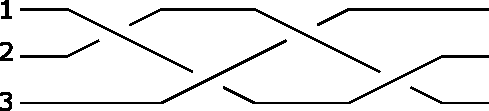
\includegraphics{Figures/3-strands.pdf}
  \caption{Three Strand Braid, ($\sigma^{-1}_1\sigma_2$) Repeated}
  \label{fig:3Strand}
\end{figure}

\subsubsection{Procedure}
\begin{itemize}
  \item Divide the dough into three equal lumps.
  \item Roll each lump into long strand.
  \item Lay the strands side-by-side and squeeze one end together.
  \item Move the top strand over the middle strand ($\sigma^{-1}_1$), then move the bottom strand over the middle strand ($\sigma_2$).
  \item Repeat ($\sigma^{-1}_1\sigma_2$) until the end of the strands is reached.
  \item Squeeze the last end together.
\end{itemize}

\subsection{Four Strands}
There are probably multiple ways to do four or more strand braids.  I'm just listing the ones that I've used.
\subsubsection{Procedure}
\begin{itemize}
  \item Divide the dough into four equal lumps.
  \item Roll each lump into long strand.
  \item Lay the strands side-by-side and squeeze one end together.
  \item Move the top strand over the adjacent strand, and under the next strand ($\sigma^{-1}_1\sigma_2\sigma^{-1}_3$).
  \item Repeat ($\sigma^{-1}_1\sigma_2\sigma^{-1}_3$) until the end of the strands is reached.
  \item Squeeze the last end together.
\end{itemize}

\subsection{Five Strands}
\subsubsection{Procedure}
\begin{itemize}
  \item Divide the dough into five equal lumps.
  \item Roll each lump into long strand.
  \item Lay the strands side-by-side and squeeze one end together.
  \item Move the top strand over the adjacent strand, and under the next strand (1:O2,U3).
  \item Move the bottom strand over the adjacent strand, and under the next strand (5:O4,U3).
  \item Repeat (alternating 1:O2,U3 and 5:O4,U3) until the end of the strands is reached.
  \item Squeeze the last end together.
\end{itemize}


\end{document}
